\section{MA-ROPE: Algorithm Design}

\Cref{fig:mdp_formulation} summarizes the MA-ROPE MDP formulation.

\begin{figure}[htbp]
\centering
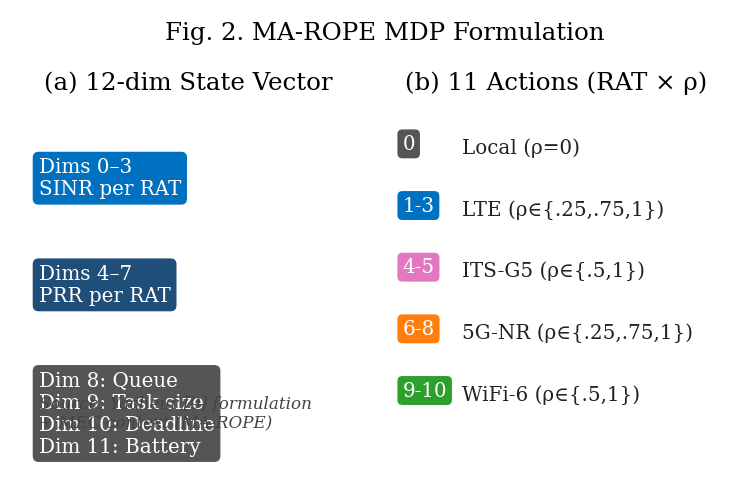
\includegraphics[width=0.45\textwidth]{figures/image4.png}
\caption{MA-ROPE MDP Formulation: 12-dimensional state space and 11-action implementation.}
\label{fig:mdp_formulation}
\end{figure}

\subsection{State and Action Space}

Following Yacheur et al. \cite{yacheur2023}, each agent observes a 12-dimensional state vector with per-RAT channel quality plus MEC context (\Cref{eq:state}). This per-RAT formulation directly enables the DQN to select the optimal RAT based on observed channel conditions---absent from prior single-SINR state designs.

\begin{equation}
\label{eq:state}
\begin{aligned}
s &= [\text{SINR}_{LTE}, \text{SINR}_{ITS}, \text{SINR}_{WiFi}, \text{SINR}_{5G}, \\
  &\quad \text{PRR}_{LTE}, \text{PRR}_{ITS}, \text{PRR}_{WiFi}, \text{PRR}_{5G}, Q, D, L, B]
\end{aligned}
\end{equation}

Each agent selects from 11 implemented discrete actions spanning local execution and selected RAT-$\rho$ pairs across LTE, ITS-G5, WiFi-6, and 5G-NR. The nominal $\rho$ is modulated by channel quality following Yacheur Division Mode \cite{yacheur2023} Algorithm 2:

\begin{equation}
\label{eq:rho_final}
\rho_{final} = \text{base\_}\rho \cdot \left(0.5 + \frac{\text{SINR\_lin}[r]}{\sum \text{SINR\_lin}[\text{all}]}\right)
\end{equation}

\subsection{Dueling Double DQN}

The Q-value is decomposed as $Q(s,a) = V(s) + A(s,a) - \text{mean}_{a'} A(s,a')$ where $V(s)$ is state value and $A(s,a)$ is advantage. Double DQN decouples action selection from target evaluation:

\begin{equation}
\label{eq:ddqn}
y = r + \gamma \cdot Q_{tgt}(s', \text{argmax}_{a'} Q_{online}(s', a'))
\end{equation}

Architecture: Linear(12->256)->ReLU->Linear(256->256)->ReLU, split into value head Linear(256->128->1) and advantage head Linear(256->128->11) for the implemented action set.

\subsection{FedAvg Cooperative Learning}

At the end of each episode, each agent i uploads local model weights $w_i$. The global model is aggregated as:

\begin{equation}
\label{eq:fedavg}
w_{global} = \sum_i \frac{n_i}{N} \cdot w_i, \text{ participation } \geq 70\%
\end{equation}

Privacy analysis: FedAvg shares model weights instead of raw vehicle observations. This reduces data exposure relative to centralized MADDPG, but model updates can still leak information under gradient-inversion or membership-inference attacks. Production deployments should pair FedAvg with secure aggregation, access control, and/or differential privacy; in this paper MADDPG is treated as a performance upper bound with stronger data-sharing assumptions.

\begin{algorithm}[htbp]
\caption{MA-ROPE Training with FedAvg}
\label{alg:ma_rope}
\begin{algorithmic}[1]
\REQUIRE $N$ agents, episodes $E$, participation threshold $\tau=0.70$
\STATE Initialize $w_i$ for each agent $i$, replay buffers $B_i$
\FOR{episode $e = 1$ to $E$}
    \FOR{each step $t$}
        \STATE $s_t \leftarrow \text{observe}()$ \COMMENT{12-dim per-RAT state (\Cref{eq:state})}
        \STATE $a_t \leftarrow \varepsilon\text{-greedy}(Q_{online}(s_t))$
        \STATE apply SINR-proportional $\rho$ (\Cref{eq:rho_final})
        \STATE execute $a_t$; receive $r_t = U (\text{\Cref{eq:utility_all}}), s_{t+1}$
        \STATE store $(s_t, a_t, r_t, s_{t+1})$ in $B_i$
        \STATE sample minibatch; update $Q_{online}$ via (\Cref{eq:ddqn})
    \ENDFOR
    \IF{$|\text{participants}| / N \geq \tau$}
        \STATE $w_{global} \leftarrow \sum \frac{n_i}{N} \cdot w_i$ \COMMENT{FedAvg aggregation (\Cref{eq:fedavg})}
        \STATE broadcast $w_{global} \rightarrow \text{all agents}$
    \ENDIF
\ENDFOR
\end{algorithmic}
\end{algorithm}
